\section{アジャイルソフトウェア開発の実践方法}

アジャイルソフトウェア開発を導入する理由として、4つの仮定があることを前節で示した。その4つの仮定を満たすために、アジャイルソフトウェア開発手法では大きく分け以下の3つについて言及している。

\begin{enumerate}
  \item アジャイルソフトウェア開発における開発工程
  \item 開発工程を実行するチーム
  \item チームが習慣づけるべき開発技法
\end{enumerate}

\subsection{アジャイルソフトウェア開発における開発工程}

開発工程はウォーターフォール\ref{fig:waterfall}と異なり、1〜4週間の期間で要求分析、設計、実装、テストを行い、その期間を何度も繰り返す\ref{fig:agile}ことによってソフトウェアを開発して行く。またこの1〜4週間の期間のことをイテレーション (もしくはスプリント)\footnote{アジャイルにおける繰り返しの1単位をイテレーション、スプリント、または別の呼び方のどれで呼ぶかは、アジャイルソフトウェア開発の中でもXPやスクラムと呼ばれる更に細分化された手法のうち、どれを採用するかによって変わる。}と呼ぶ。

\begin{figure}[H]
\centering
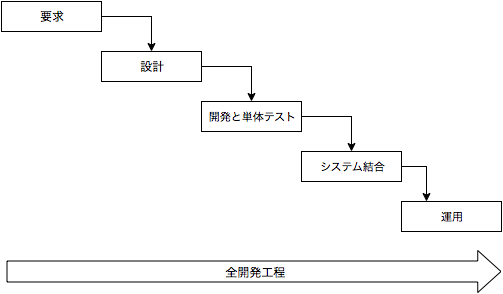
\includegraphics[height=8cm]{./assets/images/waterfall.png}
\caption{ウォーターフォール開発の開発工程}
\label{fig:waterfall}
\end{figure}

\begin{figure}[H]
\centering
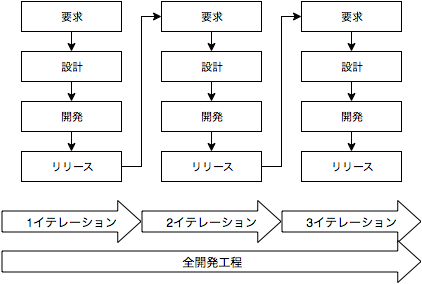
\includegraphics[height=8cm]{./assets/images/agile.png}
\caption{アジャイルソフトウェア開発の開発工程}
\label{fig:agile}
\end{figure}


\subsection{開発工程を実行するチーム}


アジャイルにおいての開発チームは、上記の開発工程に沿って、ソフトウェア開発で起きた問題を解決する為に組織される。そのため組織されるメンバーは開発に関わる全ての工程をまかなうことが可能であるかつ、メンバー個々人は開発に必要な能力を横断的に有している事が求められる。つまり、ウォーターフォール開発を行っていた開発チームは、アジャイル開発を始めようとする際は大きな組織変更が必要かつ、場合によってはアジャイル開発のチームメンバーとしての要求を満たさない人員が発生する可能性がある。しかし、アジャイルにおいての開発メンバーとして要求される両方の条件を満たしていると開発チームは一丸となってソフトウェア開発で起きる問題を解決する努力ができる。

\subsection{チームが習慣づけるべき開発技法}


文献中 (アジャイルサムライ) 中で、開発チームが定められたイテレーション内で実行すべき (習慣づけるべき) とされている開発技法は以下が挙げられる。

\begin{itemize}
 \item[・]テスト駆動開発の実践
 \item[・]継続的インテグレーション
\end{itemize}

\subsubsection{テスト駆動開発の実践}

テスト駆動開発とは、実際にプログラムを記述する際のテクニックの事を指している。これから作成するプロダクトコード\footnote{後述するテストコードとの対比として、実際に作成しなければいけないソフトウェアのコードをプロダクトコードと呼ぶ}に対して、自動で実行可能なテストコード\footnote{先述したプロダクトコードとの対比として、プロダクトをテストするためのプログラムをテストコードと呼ぶ}を先に記述し、あるべきテストコードが失敗する状態を作った後に、プロダクトコードの記述を行いテストコードが成功するようする。テストが成功したらプログラムをリファクタリング\footnote{プログラムの振舞を変えず、内部のコードを綺麗にすること}し、コードの質上げる\ref{fig:tdd}。この一連の流れはテストをサポートするためのツールが失敗する際に赤、テストが成功した時に緑色の出力をすることから、「RED, GREEN, リファクタリング」とも呼ばれる。

\begin{figure}[H]
\centering
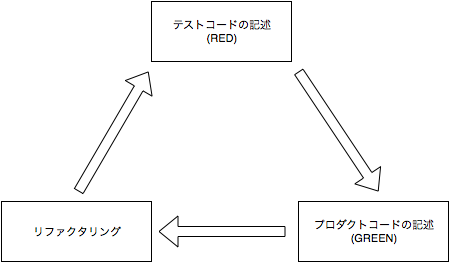
\includegraphics[height=8cm]{./assets/images/tdd.png}
\caption{テスト駆動開発}
\label{fig:tdd}
\end{figure}


このテスト駆動開発を実践することにより得られるメリットは3つある。1つめはプロダクトコードに対して無駄なバグを混入させることを減らすこと、2つめはプロダクトコードを変更した際の影響を素早く確認ができる。3つめでメリットとして最も大きいことは、作成したプログラムが安定していること確認できることによって安心感を得られることである。

\subsubsection{継続的インテグレーション}

継続的インテグレーションとは

\begin{quote}

  開発者がソフトウェアに加えた変更を取り込んで、ソフトウェア全体として統合する作業を途切れること無く続けていく取り組みのことを、継続的インテグレーションと呼ぶ。

\end{quote}

と文献\cite{西村直人2011アジャイルサムライ}の中で述べられている。つまりソフトウェア開発の1フェーズとして、コードの統合フェーズを設けることなく、日常的にソフトウェアを統合することを指し、そのためには、ソースコードのバージョン管理システム\footnote{バージョン管理システムとは、開発し日々更新されるソフトウェアに対してバージョンを振ることが出来、また特定のバージョンからの派生や、派生したバージョンの統合をサポートする。}や、ソフトウェアのビルドの自動化\footnote{ビルドとは、ソフトウェアのコンパイルのみならず、使用ライブラリの依存関係解決やDBのスキーマ管理などが含まれる}などが求められる。 (図を用意する)
